\documentclass{article}
\usepackage{graphicx}
\usepackage{subcaption}
\usepackage{geometry}
\usepackage{tikz}
\usepackage{amsmath}
\usepackage{cleveref}
\usepackage{float}
\usepackage[useregional]{datetime2}
\usepackage{url}
\def\checkmark{\tikz\fill[scale=0.4](0,.35) -- (.25,0) -- (1,.7) -- (.25,.15) -- cycle;}
\usepackage[font=small,skip=0pt]{caption}
\geometry{legalpaper, margin=1in}
\title{STAT 8003 Project 1}
\author{Zhijia Chen}
\date{\today}

\begin{document}

\begin{titlepage}
    \maketitle
\end{titlepage}

\textbf{Summary}

Stock performance forecast is always an intriguing topic. Many indexes has been proposed as indicator for the market performance, within which the S\&P 500 index is arguably the most widely recognized. The S\&P 500 index is a composite index of 500 largest U.S. stocks and it generally shows the overall performance of the whole stock market.Thus S\&P 500 prediction is of great interests in the field of market forecast. While predicting S\&P 500 based on relevant variables might produce a stable model that is more tolerant of market disturbance, it requires a deep insight of the market and tremendous efforts in sorting out accurate relationships between the index and it's dependent variables, predicting the future of the S\&P 500 solely based on it's past, however, is a much simpler method. In this study, we show that ARMA model, or Autoregressive Moving Average model, is able to fit the S\&P 500 annual returns very well, and can also produce a reliable prediction of changes in the near future. We used the returns after 1950 to fit the ARMA model and use the last 12 months (Jan, 2017 - Dec, 2017) to test the forecast. The AIC and BIC for the model are pretty low, with the former being -2.067e+03 and and the later being -1.988e+03. But we do notice that the changes in the fitted data usually lag behind the actual data, and the error of the forecast data increases as the forecast span increases. The ARMA model might not able to produce an accurate prediction, especially when there are dramatic changes, but when only the short time trend is of interest, it's much more efficient compared to those modeling methods such as linear regression that requires finding the dependent variables of the target variable and the corresponding relationships.

\vspace{\baselineskip}
\textbf{Model Introduction}

In this study, our goal is to model the annual returns of the S\&P 500 index after 1950. We use the ARMA model to fit the data of the first 50 years, i.e. 1950~2000, and try to do a 1-year-span forecast. An ARMA model, or Autoregressive Moving Average model, is used to describe weakly stationary stochastic time series in terms of two polynomials. The first of these polynomials is for autoregression, the second for the moving average\cite{arma}. The model is usually referred as the $ARMA(p,q)$ Model, where $p$ is the order of the autoregressive polynomial and q is the order of the moving average polynomial. The model is given by:

\begin{align*}
    X_t=c+\epsilon_t+\sum_{i=1}^p\phi X_{t-i}+\sum_{i=1}^q\theta_i\epsilon_{t-i}
\end{align*}

Where:
\begin{itemize}
    \item $\phi$ is the autoregressive model's parameters.
    \item $\theta$ is the moving average model's parameters.
    \item c is a constant.
    \item $\epsilon_t$ is the prediction error at time $t$.
\end{itemize}

\textbf{Exploratory Data Analysis}

Figure ~\ref{fig:returns} shows the S\&P 500 annual returns After 1950. We perform a augmented Dickey-Fuller test on the data and the alternative hypothesis indicates that the annual returns is a stationary time series. Figure ~\ref{fig:adf} shows the test result produced by the adf.test function in R.

\begin{figure}[H]
    \centering
    \begin{subfigure}{.5\textwidth}
        \centering
        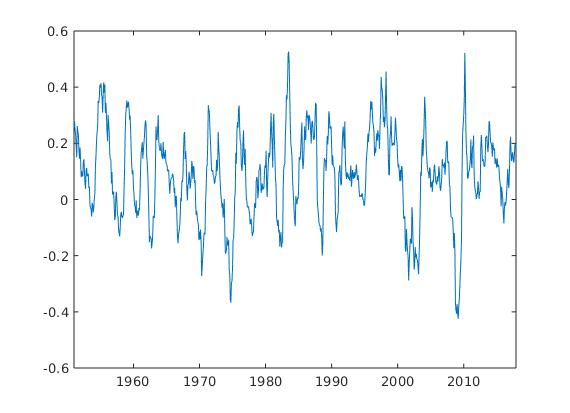
\includegraphics[width=1\textwidth]{sp500-annual-increase.jpg}
        \caption{S\&P 500 Annual Returns After 1950}
        \label{fig:returns}
    \end{subfigure}%
    \begin{subfigure}{.5\textwidth}
        \centering
        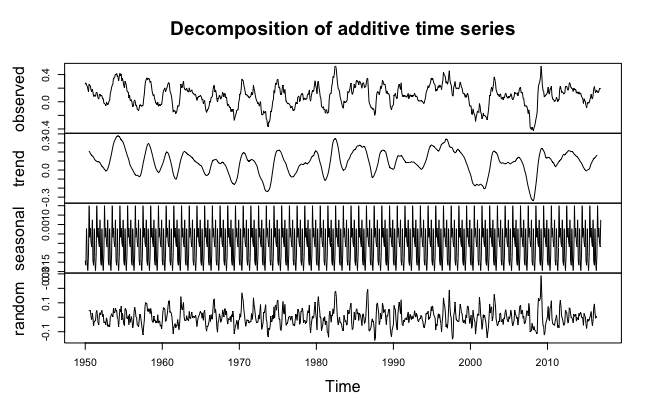
\includegraphics[width=1\textwidth]{stationary-test.png}
        \caption{Augmented Dickey-Fuller Test}
        \label{fig:adf}
    \end{subfigure}
    %\caption{A figure with two subfigures}
    %\label{fig:test}
\end{figure}

\vspace{\baselineskip}
\textbf{Model Development and Test}

The most important step in building the $ARMA(p, q)$ model is selecting the autoregression lag order $p$ and the moving average lag order $q$. As we use the MATLAB Econometrics Toolbox to build the model, we follow it's documentation\cite{lags} to plot autocorrelation function(ACF) and partial autocorrelation function to choose potential lags. We also compute the mean of the returns to estimate the constant $c$.

Figure ~\ref{fig:acf} and figure ~\ref{fig:pacf} show the autocorrelation function and partial autocorrelation function of the S\&P 500 annual returns respectively. In the ACF plot, we see that the function shuts off at lag 10, so we choose the first 10 lags as potential lags for the moving average model. And similarly, we only choose those lags that exceeds the confidence bounds (marked by the blue lines) as potential values (1, 2, 4, 5, 6, 9, 10, 13, 14, 25) for the autoregression model.

\begin{figure}
    \centering
    \begin{subfigure}{.5\textwidth}
        \centering
        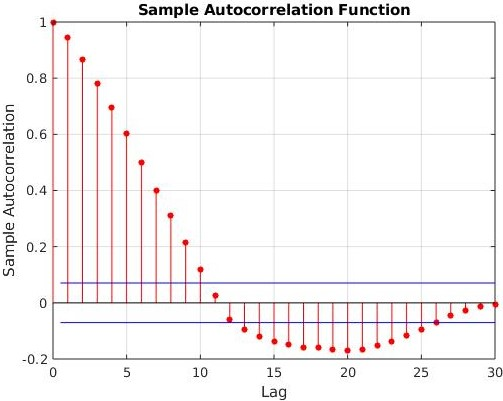
\includegraphics[width=1\textwidth]{acf.jpg}
        \caption{autocorrelation function plot}
        \label{fig:acf}
    \end{subfigure}%
    \begin{subfigure}{.5\textwidth}
        \centering
        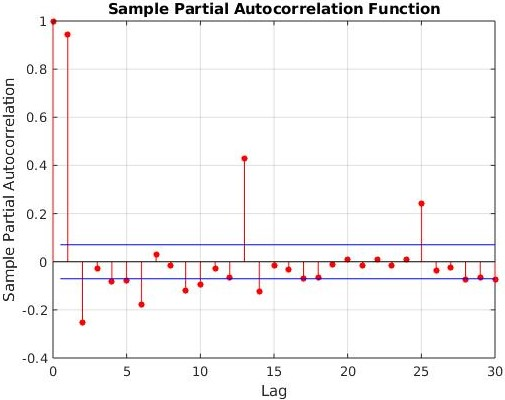
\includegraphics[width=1\textwidth]{pacf.jpg}
        \caption{partial autocorrelation function plot}
        \label{fig:pacf}
    \end{subfigure}
    %\caption{A figure with two subfigures}
    %\label{fig:test}
\end{figure}

With potential lags chosen above, we explore the best best combination of the autoregression lags and moving averages lags for model. However, there are $2^{20}$ possible combinations of the choose lags which is impossible for us to do a brutal search, thus we loop through 1 to 10 for the autoregression lag order $p$ and loop through 1 to 25 for the moving average lag order $q$. In each loop of $p_i$ and $q_j$, if both $p_i$ and $q_j$ are in the potential lags for their corresponding models, we then estimate the $ARMA(p_i, q_j)$ model with the chosen lags that within the order using maximum likelihood method. Thus we only need to explore $10\times10=100$ combinations of the lags. Finally, we choose the model that has the minium AIC as our final model which is given below (all the coefficients are rounded to 3 decimal places):

\begin{align*}
    X_t=&0.015X_{t-1}+0.678X_{t-2}-0.602X_{t-4}+0.147X_{t-5}+\\
        &0.263X_{t-6}+0.062X_{t-9}-0.056X_{t-10}-0.153X_{t-13}-0.089X_{t-14}+\\
        &1.108\epsilon_{t-1}+0.261\epsilon_{t-2}+0.140\epsilon_{t-3}+1\epsilon_{t-4}+1\epsilon_{t-5}+\\
        &0.213\epsilon_{t-6}+0.051\epsilon_{t-7}+0.640\epsilon_{t-8}+0.674\epsilon_{t-9}+\\
        &0.10152+\epsilon_t\\
\end{align*}

Figure ~\ref{fig:fit} shows the fitted data and the residual plot. We can see that the model fits the data very well with maximum residual at only around 0.15. The AIC and BIC for the model are also at a very low level which are -2.0673e+03 and -1.9882e+03 respectively.

\begin{figure}[h!]
    \centering
    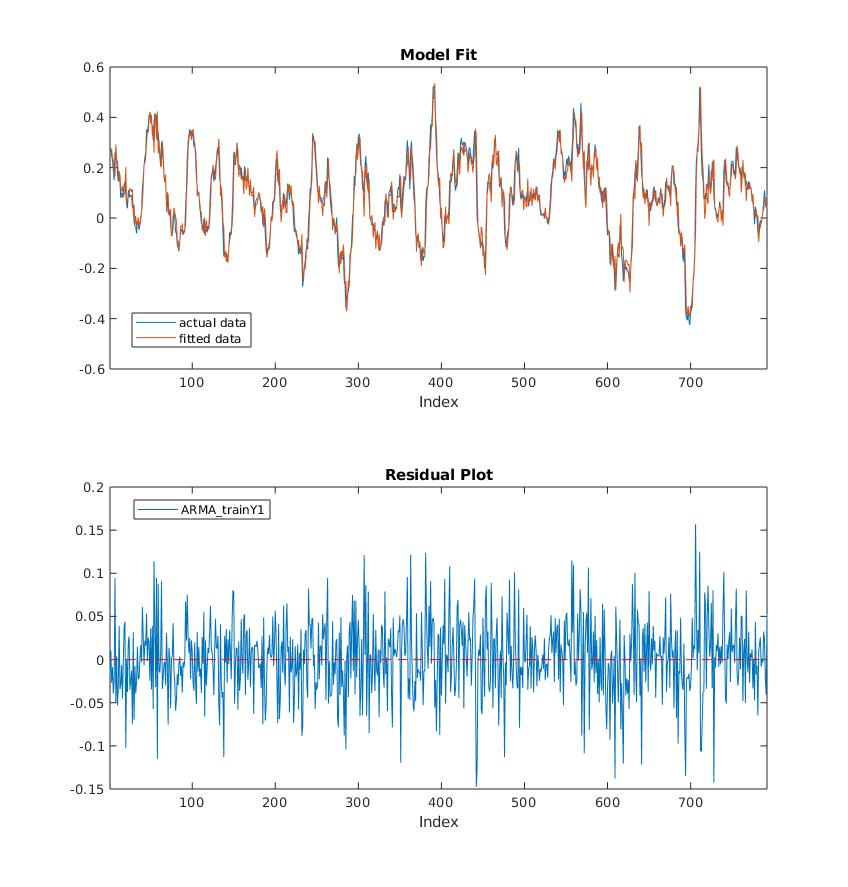
\includegraphics[width=0.5\textwidth]{fit.jpg}
    \caption{the fitted data and residual plot of the best model}
    \label{fig:fit}
\end{figure}

To test our model, we do a 1-year span forecast and compare it against the actual data. Figure ~\ref{fig:forecast1} presents the forecast data and the error. We notice that the change trend of the forecast generally matches the actual data, but the data change scale diminishes as the time goes which makes the future predication approaching to a constant. Figure ~\ref{fig:forecast10} shows a 10-year forecast and the predicated data indeed level off after 3 years. Overall, the results show that our model is capable of doing a good short term forecast but would need further improvements to increase the reliable forecast span.

\begin{figure}[H]
    \centering
    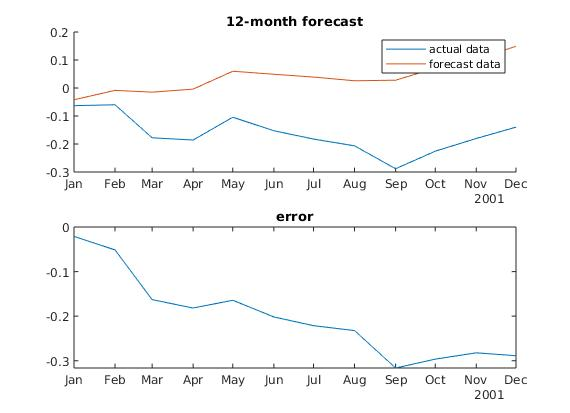
\includegraphics[width=0.5\textwidth]{forecast-1-year.jpg}
    \caption{1-year span forecast data and the forecast error}
    \label{fig:forecast1}
\end{figure}

\begin{figure}[H]
    \centering
    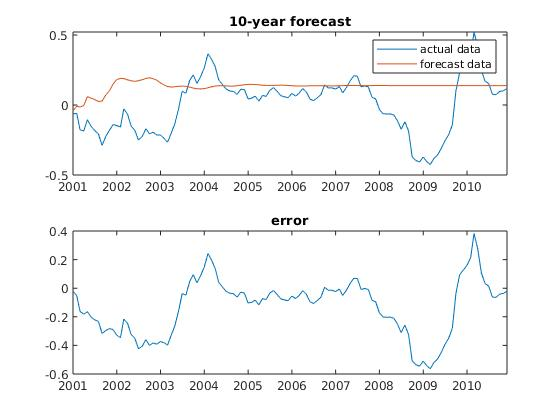
\includegraphics[width=0.5\textwidth]{forecast-10-year.jpg}
    \caption{1-year span forecast data and the forecast error}
    \label{fig:forecast10}
\end{figure}

\bibliography{project1} 
\bibliographystyle{ieeetr}
\end{document}

